% Provenance (never printed): cycle 4 SVT/physique, "La planete Terre,
% l'environnement": the atmosphere, its structure and its layers, pressure
% and altitude, the ozone layer; see sources/book1/PROVENANCE.md. Book 1,
% grade 8, chapter 1.
% Vocabulary guard: owns the layers of the atmosphere (troposphere,
% tropopause, stratosphere, mesosphere, thermosphere), the environmental
% lapse rate and the ozone layer. Air pressure and the barometer are the
% physics books' (recalled), the composition of air and ozone the molecule
% the chemistry books'; "convection cell" is g8.2's and is not used here;
% adiabatic cooling is Book 2's.
\chapter{Atmosfer}\label{ch:g8:the-atmosphere}

Di sebuah \omterm{def:g4:clouds-rain-snow:weather-station}{stasiun cuaca}, sesaat sebelum jam yang telah disepakati, seorang
ahli meteorologi berjalan ke luar di atas rumput sambil memegang sebuah
balon berisi hidrogen atau helium, yang lebarnya kira-kira \qty{1.5}{m}.
Di bawahnya, pada seutas tali yang panjang, tergantung sebuah parasut
oranye kecil dan sebuah kotak alat seberat 60 sampai 80 gram: sebuah
\emph{radiosonde}. Ia melepaskannya. Balon itu naik kira-kira \qty{300}{m}
setiap menit, dan setiap detik radiosonde itu mengirimkan lewat radio
tekanan, suhu, kelembapan, dan posisinya. Selagi naik, balon itu
menggembung, sampai lebarnya 6 sampai \qty{8}{m} lalu meletus, sering
lebih dari \qty{30}{km} di atas tanah, dua jam sesudah peluncuran. Pada
jam-jam yang sama setiap hari, adegan yang sama terjadi di lebih dari 800
stasiun di seluruh dunia.
% ledger: nws:radiosonde

\begin{omfigure}
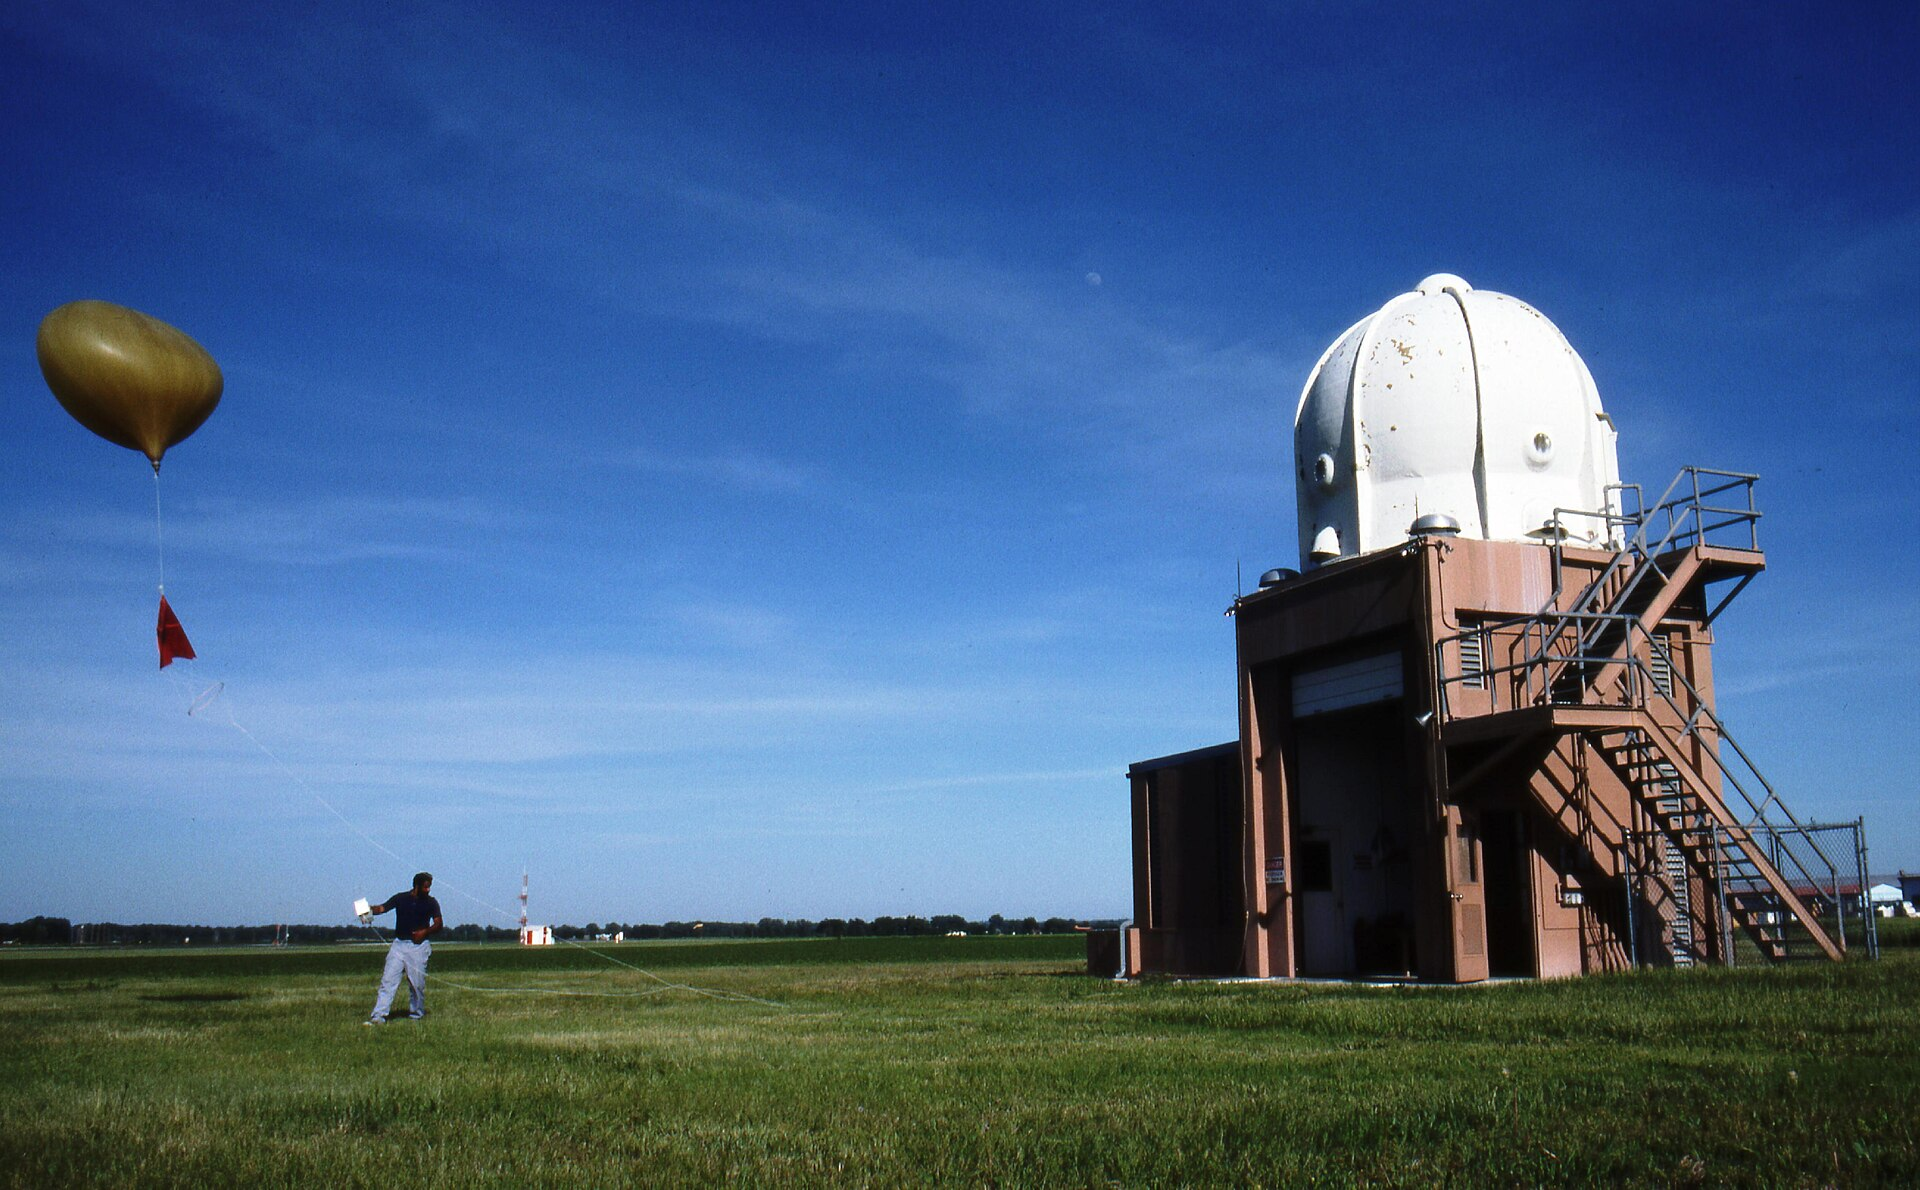
\includegraphics[width=0.78\linewidth]{images/book1/g8-radiosonde-launch.jpg}

{\small Peluncuran balon \omterm{def:g1:watching-the-weather:weather}{cuaca} di Topeka, Kansas (Amerika Serikat):
parasut (merah) dan radiosonde tergantung di bawah balon. Foto karya
Stephen Corfidi, NOAA/National Weather Service (domain publik, melalui
Wikimedia Commons).}
% ledger: commons:radiosonde-launch
\label{fig:g8:the-atmosphere:launch}
\end{omfigure}

Mengapa balon itu menggembung selagi naik? Apa yang diukur radiosonde
dalam perjalanannya ke atas, dan mengapa suhunya tidak terus-menerus turun
saja? Di mana udara berakhir?

\begin{recall}
Yang disebut \emph{atmosfer} adalah lapisan udara yang menyelubungi Bumi.
Udara menekan segala sesuatu yang disentuhnya: inilah \emph{tekanan udara},
yang diukur dengan barometer (buku-buku fisika). Dinas \omterm{def:g1:watching-the-weather:weather}{cuaca} menyatakannya
dalam hektopascal (hPa); di \omterm{def:g4:world-physical-map:altitude}{permukaan laut} besarnya kira-kira
\qty{1013}{hPa}. Udara kering terdiri atas kira-kira 78~\% nitrogen dan
21~\% oksigen, dengan sedikit argon, karbon dioksida, dan gas-gas lain
(buku-buku kimia). \omterm{def:g4:clouds-rain-snow:cloud}{Awan} terdiri atas tetes-tetes air yang sangat kecil
atau kristal-kristal es (\cref{ch:g4:clouds-rain-snow}).
\end{recall}
% ledger: air:N2, air:O2, ussa76:sea-level

\section{Selubung yang tipis}

Dilihat dari Stasiun Antariksa Internasional, atmosfer adalah garis tipis
yang bercahaya di sepanjang tepi Bumi. Sebagian besar udara, dan hampir
semua \omterm{def:g4:clouds-rain-snow:cloud}{awan}, berada di beberapa kilometer terbawahnya.
% ledger: commons:iss-sunset

\begin{omfigure}
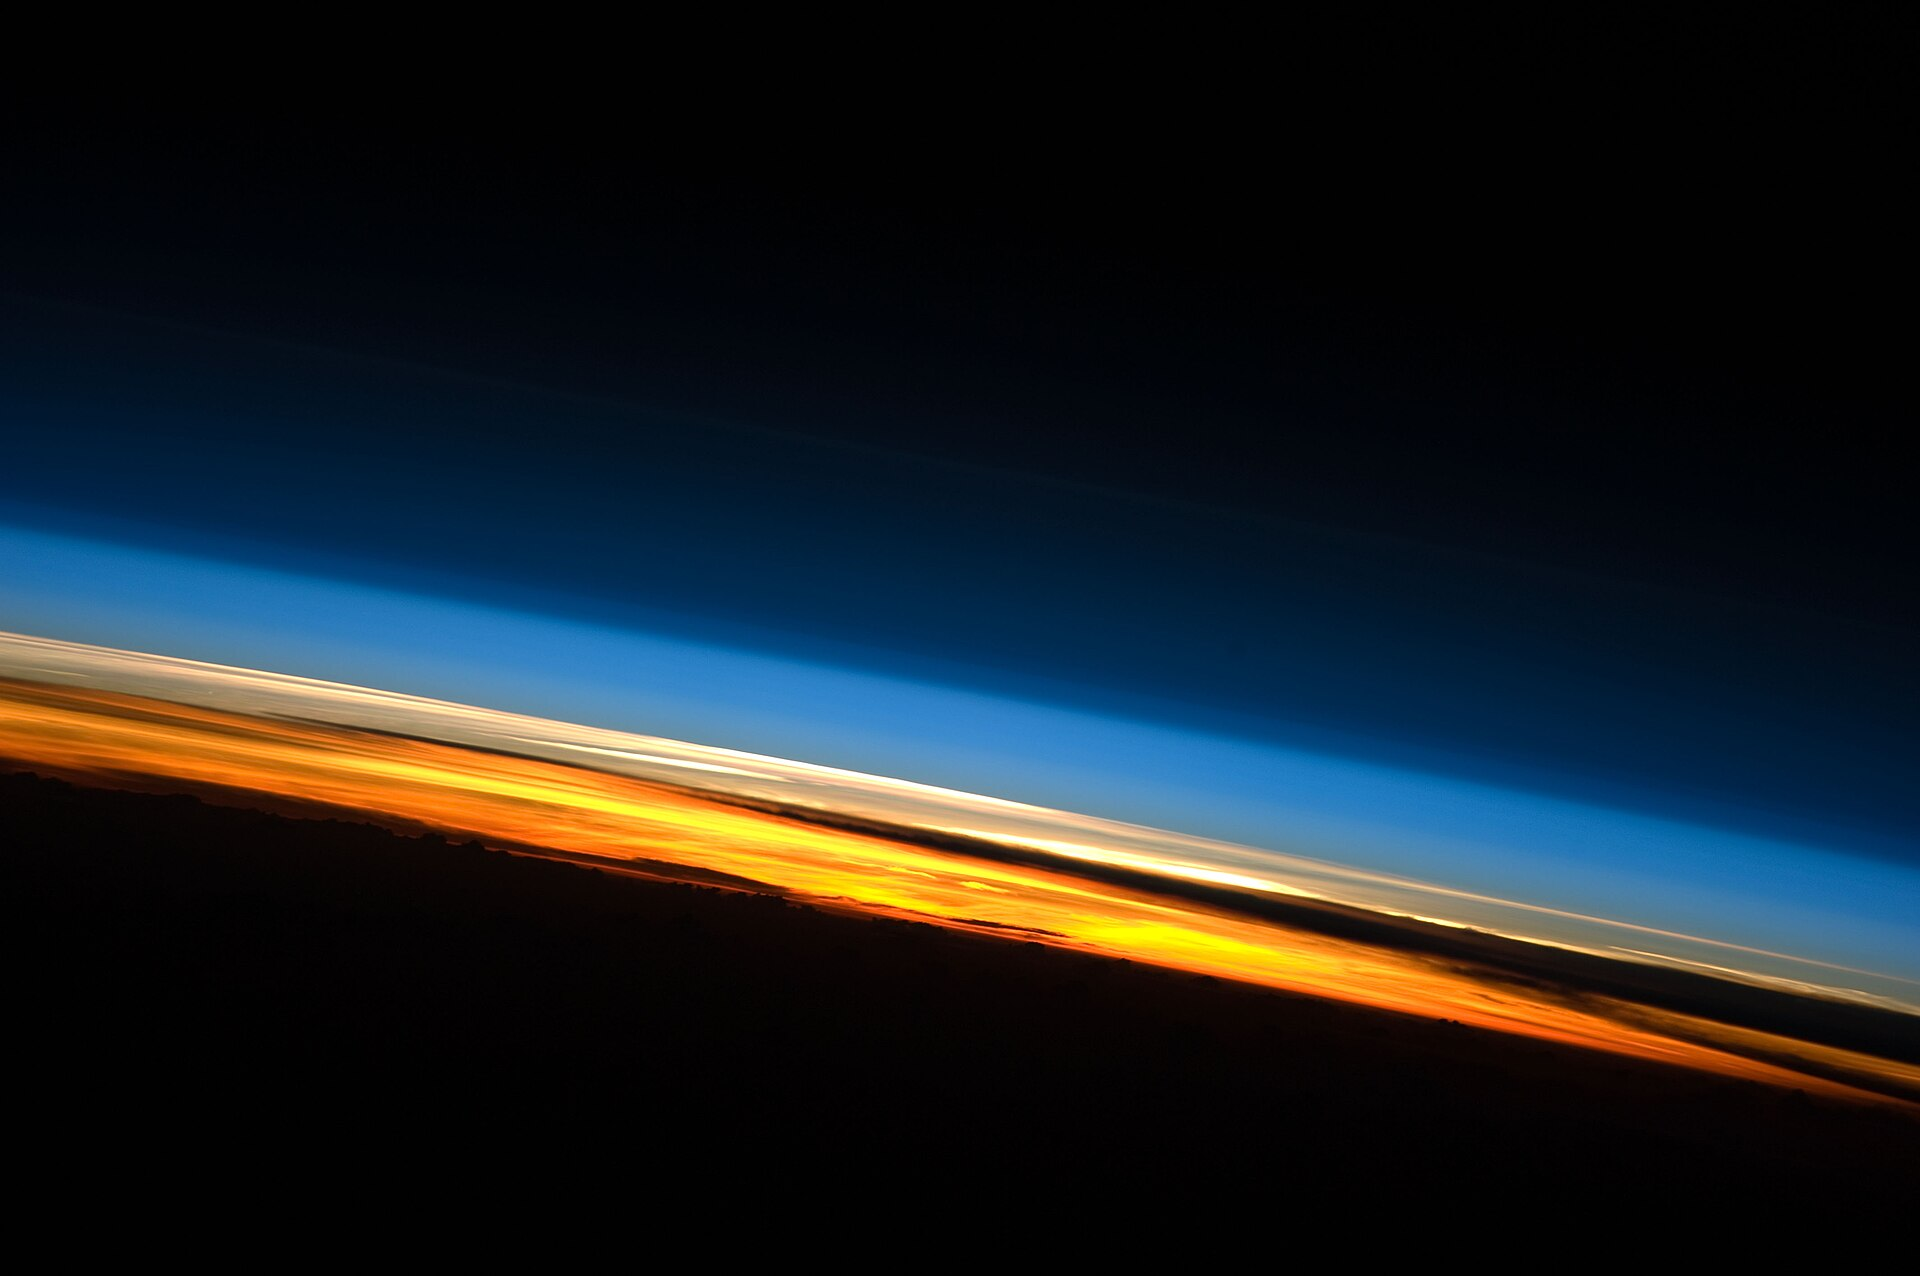
\includegraphics[width=0.78\linewidth]{images/book1/g8-iss-limb.jpg}

{\small Tepi Bumi pada saat matahari terbenam, difoto dari Stasiun
Antariksa Internasional di atas \omterm{def:g2:water-on-earth:ocean}{Samudra} Hindia pada tanggal 14~Juni 2010.
Pita oranye dan kuning adalah lapisan terbawah atmosfer, dengan \omterm{def:g4:clouds-rain-snow:cloud}{awan-awannya}
yang gelap; di atasnya terdapat lapisan-lapisan yang lebih pucat lalu biru,
yang memudar ke dalam hitamnya antariksa. Foto NASA, Ekspedisi~23 Stasiun
Antariksa Internasional
(domain publik, melalui Wikimedia Commons).}
% ledger: commons:iss-sunset
\label{fig:g8:the-atmosphere:limb}
\end{omfigure}

Atmosfer tidak mempunyai puncak yang tajam: udaranya makin lama makin tipis
seiring \omterm{def:g4:world-physical-map:altitude}{ketinggian}. Menurut kesepakatan, antariksa dimulai kira-kira pada
\omterm{def:g4:world-physical-map:altitude}{ketinggian} \qty{100}{km}. Dibandingkan dengan jari-jari Bumi,
\qty{6371}{km}, \omterm{def:g4:world-physical-map:altitude}{ketinggian} itu sangat kecil: $100 \div
6371 \approx 0.016$, kurang dari 2~\% jari-jari. Pada sebuah \omterm{def:g3:continents-and-oceans:globe}{bola dunia} yang
lebarnya \qty{30}{cm}, seluruh atmosfer akan menjadi selaput setebal
kira-kira \qty{2}{mm}.
% ledger: ucar:layers, earth:Rmean

\begin{omfigure}
\begin{tikzpicture}[font=\footnotesize]
  % 1 cm = 100 km: the Earth's surface is a circle of radius 63.71 cm
  \def\R{63.71}
  \useasboundingbox (-6.9,-1.6) rectangle (6.9,1.0);
  \fill[blue!8] (0,-\R) ++(85:\R+1) arc (85:95:\R+1) -- ($(0,-\R)+(95:\R)$) arc (95:85:\R) -- cycle;
  \fill[omLithAlluv!70] (0,-\R) ++(85:\R) arc (85:95:\R) -- ++(0,-0.6) -- ($(0,-\R)+(85:\R)+(0,-0.6)$) -- cycle;
  \draw[black, line width=0.6pt] (0,-\R) ++(85:\R) arc (85:95:\R);
  \foreach \h/\c in {0.1102/omThm, 0.4938/omMeth, 0.86/omDef} \draw[\c, line width=0.5pt] (0,-\R) ++(85:\R+\h) arc (85:95:\R+\h);
  \draw[black!60, dashed] (0,-\R) ++(85:\R+1) arc (85:95:\R+1);
  \node[anchor=west, omThm] at (5.65,-0.14) {\qty{11}{km}};
  \node[anchor=west, omMeth] at (5.65,0.25) {\qty{49}{km}};
  \node[anchor=west, omDef] at (5.65,0.62) {\qty{86}{km}};
  \node[anchor=east, black!70] at (-5.65,0.75) {\qty{100}{km}};
  \node[anchor=north] at (0,-0.15) {permukaan Bumi};
  \draw[|-|] (-5,-1.05) -- node[below] {\qty{1000}{km}} (5,-1.05);
\end{tikzpicture}

{\small Sepotong Bumi dan atmosfernya yang digambar berskala (\qty{1}{cm}
untuk \qty{100}{km}), sampai \qty{100}{km}, batas antariksa (garis
putus-putus). Garis-garis berwarna adalah batas-batas lapisan yang dibahas
nanti dalam bab ini; lapisan terbawah, tempat semua \omterm{def:g1:watching-the-weather:weather}{cuaca} terjadi, tebalnya
hampir tidak sampai satu milimeter.}
% ledger: earth:Rmean, ucar:layers (limits: figdata/grade-8/standard_atmosphere.py main table)
\label{fig:g8:the-atmosphere:to-scale}
\end{omfigure}

\section{Tekanan turun seiring ketinggian}

Udara di bagian bawah atmosfer memikul berat seluruh udara di atasnya. Makin
tinggi kita naik, makin sedikit udara yang tersisa di atas kepala, dan
makin rendah tekanannya. Dalam model baku atmosfer yang dipakai para ahli
meteorologi dan para insinyur, tekanannya \qty{1013}{hPa} di \omterm{def:g4:world-physical-map:altitude}{permukaan
laut}, separuhnya pada \omterm{def:g4:world-physical-map:altitude}{ketinggian} kira-kira \qty{5.5}{km}, dan seperempatnya
pada kira-kira \qty{10.3}{km}.
% ledger: ussa76:sea-level, ussa76:layers (figdata/grade-8/standard_atmosphere.py main table: half_km 5.48, quarter_km 10.29)

Karena tekanan mengukur berat udara di atasnya, \omterm{def:g4:world-physical-map:altitude}{ketinggian} tempat tekanan
tinggal separuh juga merupakan \omterm{def:g4:world-physical-map:altitude}{ketinggian} yang di bawahnya terdapat separuh
dari seluruh udara: separuh atmosfer dipadatkan dalam \qty{5.5}{km}
terbawahnya. Di bawah \qty{11}{km} terdapat kira-kira 78~\% udara, di bawah
\qty{30}{km} kira-kira 99~\%.
% ledger: (computed: figdata/grade-8/standard_atmosphere.py, share_below_11km 77.7, share_below_30km 98.82)

\begin{omfigure}
\begin{minipage}[t]{0.49\linewidth}\centering
\begin{tikzpicture}
\begin{axis}[width=6.6cm, height=7.6cm, xmin=0, xmax=1100, ymin=0, ymax=30,
  xlabel={tekanan (hPa)}, ylabel={ketinggian (km)},
  tick label style={font=\scriptsize}, label style={font=\small},
  xtick={0,250,500,750,1000}, ytick={0,5,10,15,20,25,30}]
  \addplot[dashed, black!60] table {figdata/out/grade-8-standard_atmosphere-guides.dat};
  \addplot[omDef, line width=1.1pt] table[x=p_hPa, y=z_km] {figdata/out/grade-8-standard_atmosphere-pressure.dat};
  \addplot[only marks, mark=*, mark size=1.8pt, omThm] table[x=p_hPa, y=z_km] {figdata/out/grade-8-standard_atmosphere-levels.dat};
  \node[anchor=south west, font=\scriptsize, text=black] at (axis cs:506.6,5.48) {separuh};
  \node[anchor=south west, font=\scriptsize, text=black] at (axis cs:253.3,10.29) {seperempat};
\end{axis}
\end{tikzpicture}

{\small Tekanan terhadap \omterm{def:g4:world-physical-map:altitude}{ketinggian}. Tekanan tinggal separuh dari nilainya
di \omterm{def:g4:world-physical-map:altitude}{permukaan laut} pada kira-kira \qty{5.5}{km}, seperempat pada kira-kira
\qty{10.3}{km}.}
\end{minipage}\hfill
\begin{minipage}[t]{0.49\linewidth}\centering
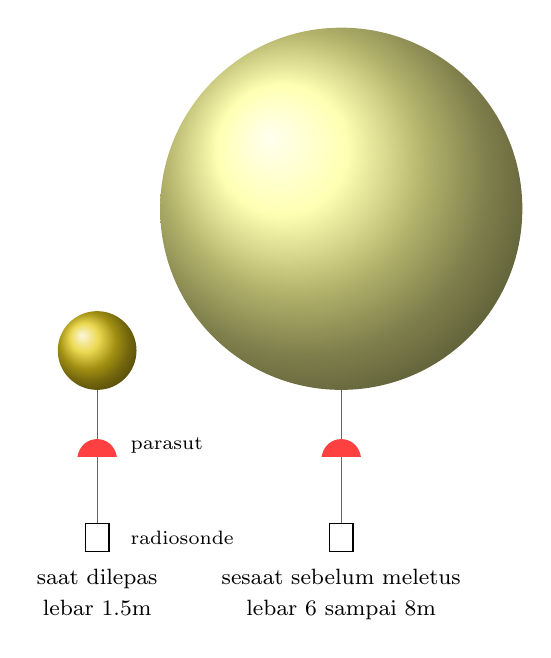
\begin{tikzpicture}[font=\footnotesize]
  % at launch: 1.5 m; at burst: about 7 m (drawn 1 cm for 1.5 m)
  \draw[black!60] (0,0.9) -- (0,2.6);
  \shade[ball color=yellow!60!brown] (0,3.1) circle (0.5);
  \fill[red!75] (-0.25,1.75) .. controls (-0.2,2.05) and (0.2,2.05) .. (0.25,1.75) -- cycle;
  \fill[white, draw=black] (-0.15,0.55) rectangle (0.15,0.9);
  \node[anchor=north] at (0,0.45) {saat dilepas};
  \node[anchor=north] at (0,0.05) {lebar \qty{1.5}{m}};
  \begin{scope}[xshift=3.1cm]
    \draw[black!60] (0,0.9) -- (0,2.6);
    \shade[ball color=yellow!40!white] (0,4.9) circle (2.3);
    \fill[red!75] (-0.25,1.75) .. controls (-0.2,2.05) and (0.2,2.05) .. (0.25,1.75) -- cycle;
    \fill[white, draw=black] (-0.15,0.55) rectangle (0.15,0.9);
    \node[anchor=north] at (0,0.45) {sesaat sebelum meletus};
    \node[anchor=north] at (0,0.05) {lebar 6 sampai \qty{8}{m}};
  \end{scope}
  \node[anchor=west, font=\scriptsize] at (0.3,1.9) {parasut};
  \node[anchor=west, font=\scriptsize] at (0.3,0.72) {radiosonde};
\end{tikzpicture}

{\small Balon itu menggembung selagi naik, karena udara di sekelilingnya
makin lama makin lemah menekan (balon dan parasut digambar berskala satu
terhadap yang lain, talinya diperpendek).}
% ledger: nws:radiosonde
\end{minipage}
% ledger: ussa76:sea-level, ussa76:layers (figdata/grade-8/standard_atmosphere.py parts pressure, levels, guides)
\label{fig:g8:the-atmosphere:pressure}
\end{omfigure}

Makin tinggi lagi, tekanan terus turun, kira-kira menjadi separuhnya lagi
setiap beberapa kilometer, sehingga tekanan itu segera menjadi sangat kecil.
Pangkat sepuluh adalah cara terbaik untuk menuliskannya. Pada \omterm{def:g4:world-physical-map:altitude}{ketinggian}
\qty{30}{km}, tekanannya kira-kira \qty{12}{hPa}, kurang lebih
$10^{-2}$ dari nilainya di \omterm{def:g4:world-physical-map:altitude}{permukaan laut} (seperseratus); pada \qty{50}{km},
kira-kira \qty{0.8}{hPa}, kurang lebih $10^{-3}$; pada \qty{80}{km},
kira-kira \qty{0.01}{hPa}, kurang lebih $10^{-5}$ dari tekanan di
\omterm{def:g4:world-physical-map:altitude}{permukaan laut}.
% ledger: ussa76:layers (figdata/grade-8/standard_atmosphere.py main table: p_30km 11.97, p_50km 0.798, p_80km 0.0105 hPa)

\begin{omfigure}
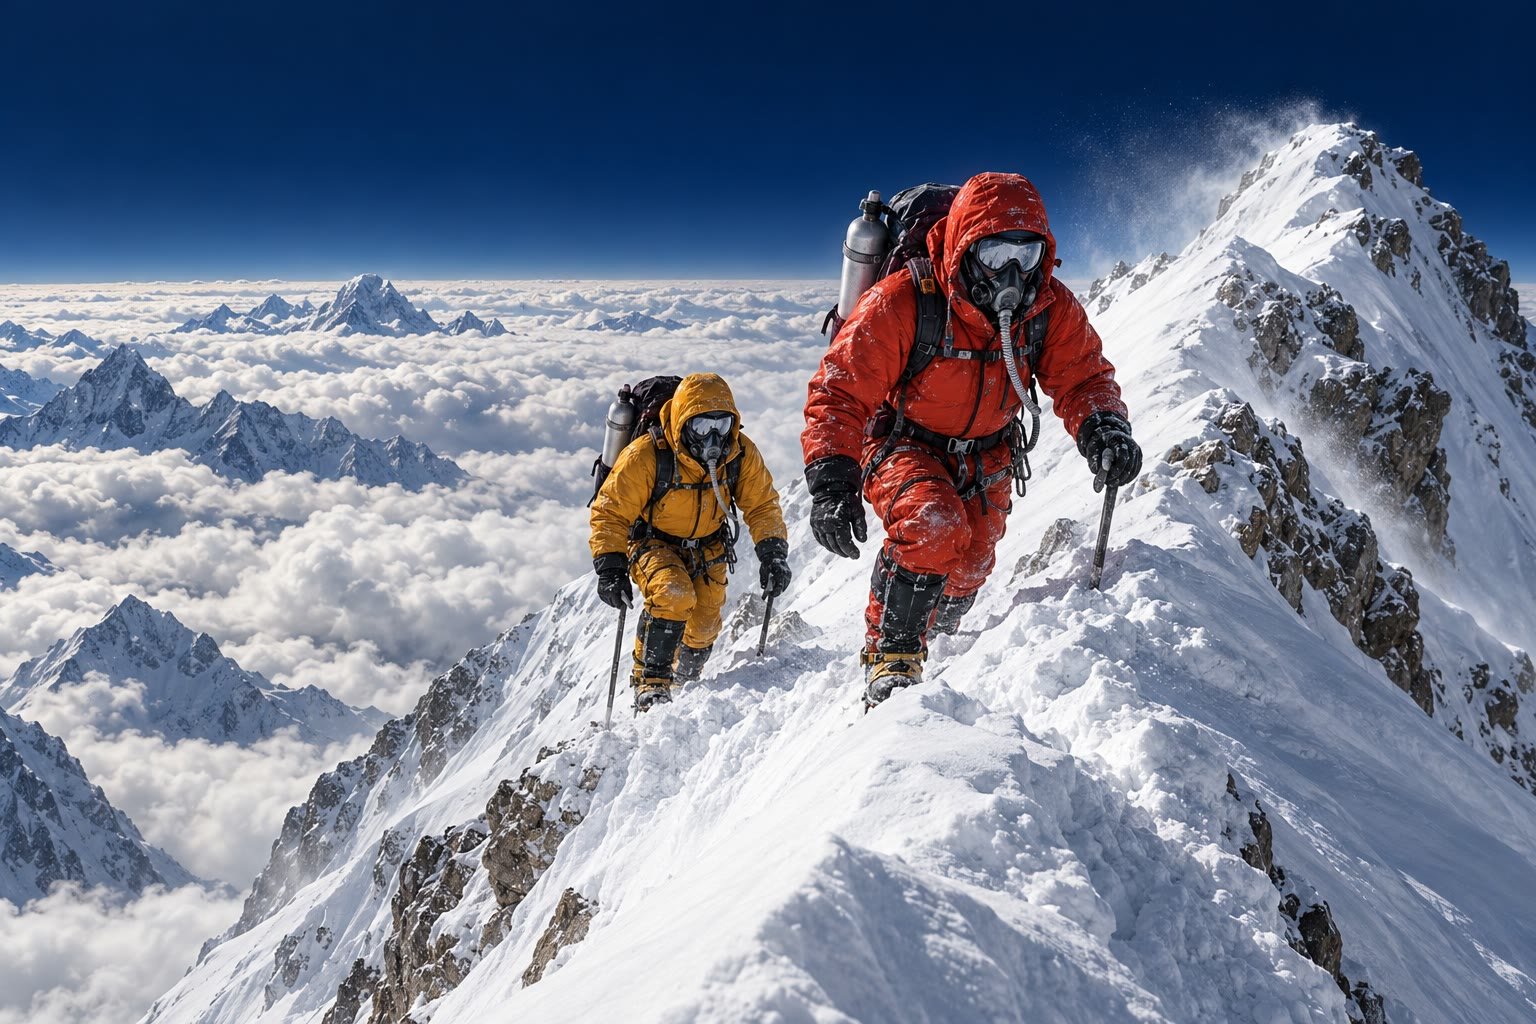
\includegraphics[width=0.5\linewidth]{images/book1/ai/g8-climbers.jpg}

{\small Para pendaki di sebuah \omterm{def:g1:landscapes-around-us:landform}{gunung} yang sangat tinggi membawa tabung
oksigen. Pada \omterm{def:g4:world-physical-map:altitude}{ketinggian} \qty{9}{km}, tekanannya kurang dari sepertiga
nilainya di \omterm{def:g4:world-physical-map:altitude}{permukaan laut}: udaranya masih mengandung 21~\% oksigen, tetapi
setiap tarikan napas menghirup jauh lebih sedikit oksigen (ilustrasi AI dari
suatu adegan umum).}
% ledger: air:O2 (figdata/grade-8/standard_atmosphere.py: pressure at 9 km 308 hPa, 30 % of sea level)
\label{fig:g8:the-atmosphere:climbers}
\end{omfigure}

\section{Suhu dan lapisan-lapisan}

Setiap orang yang pernah mendaki \omterm{def:g1:landscapes-around-us:landform}{gunung} tahu bahwa udara makin dingin
seiring \omterm{def:g4:world-physical-map:altitude}{ketinggian}. Radiosonde menunjukkan bahwa hal ini hanya benar di
bagian terbawah atmosfer. Makin tinggi lagi, suhu berhenti turun, lalu
naik, lalu turun lagi, lalu naik sekali lagi. Perubahan-perubahan ini
membagi atmosfer menjadi lapisan-lapisan.
% ledger: ucar:layers, ussa76:layers

\begin{omfigure}
\begin{tikzpicture}
\begin{axis}[width=10cm, height=9cm, xmin=-100, xmax=30, ymin=0, ymax=100,
  xlabel={suhu ($^\circ$C)}, ylabel={ketinggian (km)},
  tick label style={font=\scriptsize}, label style={font=\small},
  xtick={-100,-80,-60,-40,-20,0,20}, ytick={0,10,20,30,40,50,60,70,80,90,100}, axis on top]
  \addplot[fill=omSea!55, draw=none] table {figdata/out/grade-8-standard_atmosphere-band-troposphere.dat};
  \addplot[fill=omMeth!12, draw=none] table {figdata/out/grade-8-standard_atmosphere-band-stratosphere.dat};
  \addplot[fill=omSea!35, draw=none] table {figdata/out/grade-8-standard_atmosphere-band-mesosphere.dat};
  \addplot[fill=omThm!10, draw=none] table {figdata/out/grade-8-standard_atmosphere-band-thermosphere.dat};
  \addplot[omThm, line width=1.2pt] table[x=T_C, y=z_km] {figdata/out/grade-8-standard_atmosphere-temp.dat};
  \node[anchor=west, font=\small\bfseries, text=black!75] at (axis cs:-97,5.51) {troposfer};
  \node[anchor=west, font=\small\bfseries, text=black!75] at (axis cs:-97,30.2) {stratosfer};
  \node[anchor=west, font=\small\bfseries, text=black!75] at (axis cs:-97,67.69) {mesosfer};
  \node[anchor=west, font=\small\bfseries, text=black!75] at (axis cs:-60,93) {termosfer};
  \draw[black!50, dashed] (axis cs:-100,11.02) -- (axis cs:30,11.02);
  \draw[black!50, dashed] (axis cs:-100,49.38) -- (axis cs:30,49.38);
  \draw[black!50, dashed] (axis cs:-100,86) -- (axis cs:30,86);
  \node[anchor=south east, font=\scriptsize] at (axis cs:17,11.02) {tropopause};
  \node[anchor=south east, font=\scriptsize] at (axis cs:29,49.38) {stratopause};
  \node[anchor=south east, font=\scriptsize] at (axis cs:29,86) {mesopause};
  \fill[omMeth!45] (axis cs:19,16) rectangle (axis cs:23,48);
  \node[anchor=east, font=\scriptsize, align=right] at (axis cs:18,30) {lapisan\\ozon};
\end{axis}
\end{tikzpicture}

{\small Suhu udara terhadap \omterm{def:g4:world-physical-map:altitude}{ketinggian}, dari tanah sampai \qty{100}{km},
dalam atmosfer baku (rata-rata untuk \omterm{def:g6:latitude-longitude:latitude}{lintang} tengah). Keempat lapisan itu
diarsir; batang hijau menandai \omterm{def:g4:world-physical-map:altitude}{ketinggian} \omterm{def:g8:the-atmosphere:ozone-layer}{lapisan ozon}.}
% ledger: ussa76:sea-level, ussa76:layers, ussa76:above-86, ucar:ozone (figdata/grade-8/standard_atmosphere.py parts temp, layers, band-*)
\label{fig:g8:the-atmosphere:temperature}
\end{omfigure}

\begin{definition}[Lapisan-lapisan atmosfer]\label{def:g8:the-atmosphere:layers}
Dari tanah ke atas, atmosfer dibagi menjadi empat lapisan menurut cara
suhunya berubah seiring \omterm{def:g4:world-physical-map:altitude}{ketinggian}:
\begin{itemize}
  \item \emph{troposfer}\index{troposfer}, tempat suhu turun seiring
        \omterm{def:g4:world-physical-map:altitude}{ketinggian} dan tempat hampir semua \omterm{def:g1:watching-the-weather:weather}{cuaca} terjadi; puncaknya adalah
        \emph{tropopause}\index{tropopause};
  \item \emph{stratosfer}\index{stratosfer}, tempat suhu naik seiring
        \omterm{def:g4:world-physical-map:altitude}{ketinggian}, sampai kira-kira \qty{50}{km};
  \item \emph{mesosfer}\index{mesosfer}, tempat suhu turun lagi, sampai
        kira-kira \qty{85}{km};
  \item \emph{termosfer}\index{termosfer}, tempat udara yang sangat tipis
        makin lama makin panas seiring \omterm{def:g4:world-physical-map:altitude}{ketinggian}.
\end{itemize}
\end{definition}
% ledger: ucar:layers, ussa76:layers

\omterm{def:g8:the-atmosphere:layers}{Troposfer} menyimpan kira-kira 99~\% uap air atmosfer, sehingga hampir semua
\omterm{def:g4:clouds-rain-snow:cloud}{awan}, \omterm{def:g4:clouds-rain-snow:precipitation}{hujan}, dan \omterm{def:g4:clouds-rain-snow:precipitation}{salju} terbentuk di dalamnya. Udaranya terus-menerus
teraduk. Puncak \omterm{def:g8:the-atmosphere:layers}{troposfer} tidak sama tingginya di mana-mana: \omterm{def:g8:the-atmosphere:layers}{tropopause}
paling tinggi di atas \omterm{def:g3:continents-and-oceans:equator}{khatulistiwa}, tempat tingginya dapat mencapai
\qty{20}{km}, dan paling rendah di atas \omterm{def:g3:continents-and-oceans:poles}{kutub}, tempat tingginya dapat turun
sampai \qty{7}{km} pada musim dingin. \omterm{def:g8:the-atmosphere:layers}{Tropopause} juga lebih tinggi pada
musim panas daripada pada musim dingin. Dalam atmosfer baku, rata-rata
untuk \omterm{def:g6:latitude-longitude:latitude}{lintang} tengah, \omterm{def:g8:the-atmosphere:layers}{tropopause} terletak pada \omterm{def:g4:world-physical-map:altitude}{ketinggian} \qty{11}{km}.
% ledger: ucar:layers, ucar:tropopause, ussa76:layers

\begin{definition}[Laju penurunan suhu lingkungan]\label{def:g8:the-atmosphere:lapse-rate}
Yang disebut \emph{laju penurunan suhu lingkungan}%
\index{laju penurunan suhu lingkungan} adalah laju turunnya suhu udara seiring \omterm{def:g4:world-physical-map:altitude}{ketinggian} di dalam
\omterm{def:g8:the-atmosphere:layers}{troposfer}, dalam derajat Celsius per kilometer. Laju ini berubah dari hari
ke hari dan dari tempat ke tempat; atmosfer baku memakai rata-rata
\qty{6.5}{\degreeCelsius} per kilometer.
\end{definition}
% ledger: ussa76:layers

\begin{method}[Membaca profil suhu]\label{met:g8:the-atmosphere:profile}
\begin{enumerate}
  \item Temukan \omterm{def:g4:world-physical-map:altitude}{ketinggian} pada sumbu tegak lalu bergeraklah mendatar
        sampai ke kurva; bacalah suhu di bawahnya.
  \item Di tempat kurva condong ke kiri ketika naik, udara mendingin
        seiring \omterm{def:g4:world-physical-map:altitude}{ketinggian}; di tempat kurva condong ke kanan, udara menghangat
        seiring \omterm{def:g4:world-physical-map:altitude}{ketinggian}; di tempat kurva tegak, suhunya tidak berubah.
  \item Batas-batas antarlapisan berada di tempat kurva itu berbelok.
\end{enumerate}
\end{method}

\begin{example}[Pesawat penumpang pada ketinggian jelajah]\label{ex:g8:the-atmosphere:airliner}
Sebuah pesawat penumpang terbang jelajah pada \omterm{def:g4:world-physical-map:altitude}{ketinggian} \qty{11}{km}, di
dekat \omterm{def:g8:the-atmosphere:layers}{tropopause}. Pada profil itu, suhu di sana kira-kira
\qty{-56}{\degreeCelsius}. Dengan laju penurunan suhu: dari
\qty{15}{\degreeCelsius} di \omterm{def:g4:world-physical-map:altitude}{permukaan laut}, udara mendingin sebanyak
$6.5 \times 11 = 71.5$ derajat, sehingga suhunya $15 - 71.5 =
\qty{-56.5}{\degreeCelsius}$. Pada kurva tekanan, tekanannya kira-kira
\qty{227}{hPa}, kurang dari seperempat tekanan di tanah: kabin pesawat
harus diberi tekanan.
% ledger: ussa76:sea-level, ussa76:layers (figdata/grade-8/standard_atmosphere.py: T at 11 km -56.4 degC, p 227 hPa)
\end{example}

Di atas \omterm{def:g8:the-atmosphere:layers}{tropopause}, di dalam \omterm{def:g8:the-atmosphere:layers}{stratosfer}, pesawat penumpang mendapatkan
perjalanan yang lebih tenang: udara di sana makin hangat seiring
\omterm{def:g4:world-physical-map:altitude}{ketinggian}, sehingga udara itu tidak teraduk dari bawah. Di dalam \omterm{def:g8:the-atmosphere:layers}{mesosfer},
sebagian besar meteor terbakar habis, dan di puncaknya, dekat
\qty{86}{km}, terdapat udara yang paling dingin di seluruh atmosfer,
kira-kira \qty{-86}{\degreeCelsius}. Di dalam \omterm{def:g8:the-atmosphere:layers}{termosfer}, sinar-X dan sinar
ultraviolet Matahari memanaskan udara yang sangat tipis itu sampai ratusan,
kadang-kadang ribuan, derajat; namun udaranya begitu sedikit sehingga tidak
akan terasa hangat. Banyak satelit mengorbit Bumi di sana.
% ledger: ucar:layers, ussa76:above-86

\section{Lapisan ozon}

\omterm{def:g8:the-atmosphere:layers}{Stratosfer} makin hangat seiring \omterm{def:g4:world-physical-map:altitude}{ketinggian} karena \omterm{def:g8:the-atmosphere:layers}{stratosfer} menyerap
sebagian cahaya Matahari. Gas yang paling banyak melakukannya adalah ozon,
salah satu bentuk oksigen (kimianya dibahas dalam buku-buku kimia).

\begin{definition}[Lapisan ozon]\label{def:g8:the-atmosphere:ozone-layer}
Yang disebut \emph{lapisan ozon}\index{lapisan ozon} adalah bagian
\omterm{def:g8:the-atmosphere:layers}{stratosfer}, antara kira-kira \qty{16}{km} dan \qty{48}{km}, tempat
terdapatnya kira-kira 90~\% ozon atmosfer. Lapisan ini menyerap sebagian
besar sinar ultraviolet Matahari yang berbahaya.
\end{definition}
% ledger: ucar:ozone

Bahkan di dalam \omterm{def:g8:the-atmosphere:ozone-layer}{lapisan ozon}, ozon itu langka: hanya 1 sampai 10 molekul
dalam sejuta. Namun bersama oksigen, ozon menahan antara 95~\% dan
99.9~\% sinar ultraviolet yang mencapai Bumi, termasuk jenis-jenis yang
paling berbahaya. Energi yang diserapnya diubah menjadi panas; itulah
sebabnya suhu naik di sepanjang \omterm{def:g8:the-atmosphere:layers}{stratosfer}. Tanpa \omterm{def:g8:the-atmosphere:ozone-layer}{lapisan ozon}, sinar
ultraviolet yang mencapai tanah akan membahayakan makhluk hidup.
% ledger: ucar:ozone

\begin{inthefield}[Mengikuti balon-balon cuaca]
Dinas-dinas \omterm{def:g1:watching-the-weather:weather}{cuaca} menerbitkan hasil pengukuran radiosonde mereka, sering
berupa grafik suhu terhadap \omterm{def:g4:world-physical-map:altitude}{ketinggian} untuk setiap peluncuran. Bersama
orang dewasa, carilah hasil sondasi dari stasiun yang terdekat denganmu,
yang dibuat pukul 00.00 atau 12.00 UTC. Temukan \omterm{def:g4:world-physical-map:altitude}{ketinggian} tempat suhu
berhenti turun: itulah \omterm{def:g8:the-atmosphere:layers}{tropopause} pada hari itu. Bandingkan sondasi musim
dingin dengan sondasi musim panas.
\end{inthefield}
% ledger: nws:radiosonde, ucar:tropopause

\section{Latihan}

\begin{exercise}[$\star$]\label{exo:g8:the-atmosphere:1}
Pasangkan setiap lapisan dengan uraiannya: \omterm{def:g8:the-atmosphere:layers}{troposfer}; \omterm{def:g8:the-atmosphere:layers}{stratosfer}; \omterm{def:g8:the-atmosphere:layers}{mesosfer};
\omterm{def:g8:the-atmosphere:layers}{termosfer}. (a) Suhunya naik seiring \omterm{def:g4:world-physical-map:altitude}{ketinggian} dan \omterm{def:g8:the-atmosphere:ozone-layer}{lapisan ozon} terdapat di
sana. (b) Hampir semua \omterm{def:g1:watching-the-weather:weather}{cuaca} terjadi di sana. (c) Udara yang paling dingin
di atmosfer terdapat di puncaknya. (d) Udara yang sangat tipis dipanaskan
sampai ratusan derajat; banyak satelit mengorbit di sana.
\end{exercise}

\begin{exercise}[$\star$]\label{exo:g8:the-atmosphere:2}
Gunakan profil suhu atmosfer baku. (a) Berapa suhu di \omterm{def:g4:world-physical-map:altitude}{permukaan laut}?
(b) Pada \qty{11}{km}? (c) Pada \qty{50}{km}? (d) Pada \qty{86}{km}?
(e) Di antara \omterm{def:g4:world-physical-map:altitude}{ketinggian} berapa suhunya tidak berubah?
\end{exercise}

\begin{exercise}[$\star$]\label{exo:g8:the-atmosphere:3}
Benar atau salah? Perbaikilah kalimat yang salah. (a) Suhu udara selalu
turun seiring \omterm{def:g4:world-physical-map:altitude}{ketinggian}. (b) Separuh dari seluruh udara terdapat di bawah
kira-kira \qty{5.5}{km}. (c) \omterm{def:g8:the-atmosphere:ozone-layer}{Lapisan ozon} terdapat di dalam \omterm{def:g8:the-atmosphere:layers}{troposfer}.
(d) \omterm{def:g8:the-atmosphere:layers}{Tropopause} lebih tinggi di atas \omterm{def:g3:continents-and-oceans:equator}{khatulistiwa} daripada di atas \omterm{def:g3:continents-and-oceans:poles}{kutub}.
\end{exercise}

\begin{exercise}[$\star$]\label{exo:g8:the-atmosphere:4}
Di lapisan mana setiap benda ini berada? (a) \omterm{def:g4:clouds-rain-snow:cloud}{Awan} \omterm{def:g4:clouds-rain-snow:precipitation}{hujan}. (b) Pesawat
penumpang pada \omterm{def:g4:world-physical-map:altitude}{ketinggian} \qty{12}{km}. (c) Balon \omterm{def:g1:watching-the-weather:weather}{cuaca} sesaat sebelum
meletus, pada \qty{32}{km}. (d) Meteor yang terbakar pada \qty{75}{km}.
\end{exercise}

\begin{exercise}[$\star\star$]\label{exo:g8:the-atmosphere:5}
Pada suatu hari di musim panas, suhunya \qty{20}{\degreeCelsius} di
\omterm{def:g4:world-physical-map:altitude}{permukaan laut}. Andaikan udara mendingin \qty{6.5}{\degreeCelsius} per
kilometer. (a) Berapa suhu pada \qty{2}{km}? (b) Pada \qty{3}{km}? (c) Pada
\omterm{def:g4:world-physical-map:altitude}{ketinggian} berapa kira-kira udara mencapai \qty{0}{\degreeCelsius}?
Bulatkan sampai satu tempat desimal.
\end{exercise}

\begin{exercise}[$\star\star$]\label{exo:g8:the-atmosphere:6}
Sebuah pondok \omterm{def:g1:landscapes-around-us:landform}{gunung} terletak pada \omterm{def:g4:world-physical-map:altitude}{ketinggian} \qty{3000}{m}. Seorang
pejalan kaki berangkat dari sebuah desa pada \omterm{def:g4:world-physical-map:altitude}{ketinggian} \qty{500}{m} yang
suhunya \qty{18}{\degreeCelsius}. Dengan laju penurunan suhu
\qty{6.5}{\degreeCelsius} per kilometer: (a) Berapa kilometer pejalan kaki
itu mendaki? (b) Berapa derajat udara mendingin? (c) Suhu berapa yang
dapat diperkirakan pejalan kaki itu di pondok?
\end{exercise}

\begin{exercise}[$\star\star$]\label{exo:g8:the-atmosphere:7}
Andaikan tekanan tinggal separuhnya setiap \qty{5.5}{km}, mulai dari
\qty{1000}{hPa} di \omterm{def:g4:world-physical-map:altitude}{permukaan laut}. (a) Berapa tekanan pada \qty{5.5}{km}?
Pada \qty{11}{km}? Pada \qty{16.5}{km}? (b) Atmosfer baku memberikan
kira-kira \qty{506}{hPa}, \qty{227}{hPa}, dan \qty{96}{hPa} pada ketiga
\omterm{def:g4:world-physical-map:altitude}{ketinggian} ini (untuk \qty{1013}{hPa} di \omterm{def:g4:world-physical-map:altitude}{permukaan laut}). Apakah aturan
separuh ini baik di dekat tanah? Makin tinggi?
\end{exercise}

\begin{exercise}[$\star\star$]\label{exo:g8:the-atmosphere:8}
Di \omterm{def:g4:world-physical-map:altitude}{permukaan laut} tekanannya kira-kira \qty{1000}{hPa}, yaitu $10^3$~hPa.
(a) Pada \qty{30}{km} tekanannya kira-kira \qty{10}{hPa}. Tuliskan nilai
ini sebagai pangkat sepuluh, dan sebutkan berapa kali lebih kecil nilai itu
daripada di \omterm{def:g4:world-physical-map:altitude}{permukaan laut}. (b) Pada \qty{80}{km} tekanannya kira-kira
\qty{0.01}{hPa}. Tuliskan sebagai pangkat sepuluh. (c) Berapa kali lebih
kecil daripada di \omterm{def:g4:world-physical-map:altitude}{permukaan laut}?
\end{exercise}

\begin{exercise}[$\star\star$]\label{exo:g8:the-atmosphere:9}
Sebuah balon \omterm{def:g1:watching-the-weather:weather}{cuaca} lebarnya \qty{1.5}{m} saat diluncurkan dan \qty{6}{m}
saat meletus. (a) Berapa kali lebih lebar balon itu saat meletus?
(b) Jelaskan mengapa balon itu menggembung selagi naik. (c) Mengapa dinas
\omterm{def:g1:watching-the-weather:weather}{cuaca} menggantungkan parasut di bawahnya?
\end{exercise}

\begin{exercise}[$\star\star$]\label{exo:g8:the-atmosphere:10}
\omterm{def:g8:the-atmosphere:layers}{Tropopause} dapat mencapai \qty{20}{km} di atas \omterm{def:g3:continents-and-oceans:equator}{khatulistiwa} dan turun
sampai \qty{7}{km} di atas \omterm{def:g3:continents-and-oceans:poles}{kutub} pada musim dingin. (a) Berapa kali lebih
tebal \omterm{def:g8:the-atmosphere:layers}{troposfer} di atas \omterm{def:g3:continents-and-oceans:equator}{khatulistiwa} dalam hal ini? Bulatkan sampai satu
tempat desimal. (b) Pada profil baku, \omterm{def:g8:the-atmosphere:layers}{tropopause} berada pada \qty{11}{km}.
Apakah atmosfer baku lebih dekat ke \omterm{def:g3:continents-and-oceans:equator}{khatulistiwa} atau ke \omterm{def:g3:continents-and-oceans:poles}{kutub}? (c) Seorang
pilot terbang dari wilayah kutub ke \omterm{def:g3:continents-and-oceans:equator}{khatulistiwa} pada \omterm{def:g4:world-physical-map:altitude}{ketinggian} tetap
\qty{10}{km}. Apakah pesawat itu berada di \omterm{def:g8:the-atmosphere:layers}{troposfer} atau di \omterm{def:g8:the-atmosphere:layers}{stratosfer}
pada awal penerbangan (pada musim dingin)? Pada akhirnya?
\end{exercise}

\begin{exercise}[$\star\star\star$]\label{exo:g8:the-atmosphere:11}
Bagian dari seluruh udara yang terdapat di bawah suatu \omterm{def:g4:world-physical-map:altitude}{ketinggian} adalah
$1 - p \div
p_0$, dengan $p$ tekanan pada \omterm{def:g4:world-physical-map:altitude}{ketinggian} itu dan $p_0 =
\qty{1013}{hPa}$ tekanan di \omterm{def:g4:world-physical-map:altitude}{permukaan laut}. (a) Pada \qty{5.5}{km}, $p
\approx \qty{506}{hPa}$: berapa bagian udara yang terdapat di bawahnya?
(b) Pada \qty{11}{km}, $p \approx \qty{227}{hPa}$. (c) Pada \qty{30}{km},
$p \approx
\qty{12}{hPa}$. Berikan jawabannya dalam persen, sebagai bilangan bulat. (d) Berapa bagian udara yang terdapat di atas \qty{30}{km}?
\end{exercise}

\begin{exercise}[$\star\star\star$]\label{exo:g8:the-atmosphere:12}
Sebuah \omterm{def:g3:continents-and-oceans:globe}{bola dunia} sekolah lebarnya \qty{30}{cm}, sehingga jari-jarinya,
\qty{15}{cm}, mewakili jari-jari Bumi, \qty{6371}{km}. (a) Berapa kilometer
yang diwakili oleh \qty{1}{cm} pada \omterm{def:g3:continents-and-oceans:globe}{bola dunia} itu? Bulatkan ke kilometer
terdekat. (b) Berapa tebal, dalam milimeter, atmosfer sampai \qty{100}{km}
pada \omterm{def:g3:continents-and-oceans:globe}{bola dunia} ini? (c) Dan \omterm{def:g8:the-atmosphere:layers}{troposfer}, yang tebalnya \qty{11}{km}?
(d) Selembar kertas tebalnya kira-kira \qty{0.1}{mm}. Berapa lembar kertas
yang diperlukan untuk menyamai \omterm{def:g8:the-atmosphere:layers}{troposfer} \omterm{def:g3:continents-and-oceans:globe}{bola dunia} itu?
\end{exercise}

\section{Soal: Mengikuti balon cuaca}

\begin{problem}[{Soal akhir pekan --- sebuah balon cuaca naik menembus
atmosfer; suhu-suhunya menunjukkan lapisan-lapisan, dan tekanan-tekanannya
menunjukkan di mana tekanan tinggal seperempat dari tekanan di permukaan
laut}]
\label{pb:g8:the-atmosphere:1}
% ledger: nws:radiosonde; the table is the standard atmosphere, figdata/grade-8/standard_atmosphere.py part sonde
Sebuah radiosonde diluncurkan dari sebuah stasiun di \omterm{def:g4:world-physical-map:altitude}{permukaan laut}.
Balonnya naik kira-kira \qty{300}{m} per menit. Tabel berikut memberikan
tekanan dan suhu yang diukurnya (nilai-nilai atmosfer baku, dibulatkan).

\begin{center}\small
\begin{tabular}{|l|*{8}{c|}}
\hline
\omterm{def:g4:world-physical-map:altitude}{ketinggian} (km) & 0 & 2 & 4 & 6 & 8 & 10 & 12 & 14 \\
\hline
tekanan (hPa) & 1013 & 795 & 617 & 472 & 357 & 265 & 194 & 142 \\
\hline
suhu ($^\circ$C) & 15 & 2 & $-11$ & $-24$ & $-37$ & $-50$ & $-56$ & $-56$ \\
\hline
\hline
\omterm{def:g4:world-physical-map:altitude}{ketinggian} (km) & 16 & 18 & 20 & 22 & 24 & 26 & 28 & 30 \\
\hline
tekanan (hPa) & 104 & 76 & 55 & 40 & 30 & 22 & 16 & 12 \\
\hline
suhu ($^\circ$C) & $-56$ & $-56$ & $-56$ & $-55$ & $-53$ & $-51$ & $-49$ & $-47$ \\
\hline
\end{tabular}
\end{center}

\noindent\textbf{Bagian I --- Pendakian.}\par\nopagebreak
\begin{enumerate}[beginpenalty=10000]
  \item Berapa meter balon itu naik dalam 10 menit?
  \item Berapa lama waktu yang diperlukannya untuk mencapai \qty{6}{km}?
        Dan \qty{30}{km}?
  \item Balon itu meletus pada \qty{30}{km}. Berapa lama penerbangan itu
        berlangsung, dalam jam dan menit?
  \item Sebutkan lapisan tempat balon itu berada pada \qty{8}{km}, dan
        lapisan tempatnya berada ketika meletus.
\end{enumerate}

\noindent\textbf{Bagian II --- Suhu.}\par\nopagebreak
\begin{enumerate}[resume, beginpenalty=10000]
  \item Berapa derajat suhu turun antara tanah dan \qty{10}{km}?
  \item Berapa laju penurunan suhu dalam derajat per kilometer pada bagian
        pendakian ini?
  \item Di antara \omterm{def:g4:world-physical-map:altitude}{ketinggian} berapa suhunya tetap sama? Di mana
        \omterm{def:g8:the-atmosphere:layers}{tropopause}?
  \item Apa yang terjadi pada suhu di atas \qty{20}{km}? Gas apa yang
        menjelaskannya?
\end{enumerate}

\noindent\textbf{Bagian III --- Tekanan.}\par\nopagebreak
\begin{enumerate}[resume, beginpenalty=10000]
  \item Berapa separuh dari tekanan di \omterm{def:g4:world-physical-map:altitude}{permukaan laut}? Di antara \omterm{def:g4:world-physical-map:altitude}{ketinggian}
        berapa tekanan itu tercapai?
  \item Berapa seperempat dari tekanan di \omterm{def:g4:world-physical-map:altitude}{permukaan laut}? Bulatkan ke
        hektopascal terdekat.
  \item Di antara dua \omterm{def:g4:world-physical-map:altitude}{ketinggian} mana dalam tabel itu seperempat ini
        tercapai?
  \item Tekanan turun sebanyak \qty{71}{hPa} antara \qty{10}{km} dan
        \qty{12}{km}. Dengan menganggap tekanan itu turun secara merata,
        pada \omterm{def:g4:world-physical-map:altitude}{ketinggian} berapa kira-kira tekanannya tinggal seperempat dari
        nilainya di \omterm{def:g4:world-physical-map:altitude}{permukaan laut}? Bulatkan sampai satu tempat desimal.
\end{enumerate}
\end{problem}
